\section {Функция Bosom}
\label{TestFunctions:section:HML_TestFunction_Bosom}
\subsection {Описание функции}

\begin{tabularwide}
\textbf{Идентификатор:} & HML\_TestFunction\_Bosom. \\
\textbf{Наименование:} & Функция Bosom. \\
\textbf{Тип:} & Задача вещественной оптимизации. \\
\end{tabularwide}

\textbf{Формула} (целевая функция):
\begin{equation}
\label{TestFunctions:eq:HML_Bosom}
f\left( \bar{x}\right) = e^{\frac{z_1\left( \bar{x}_1,\bar{x}_2\right)}{1000} } +e^{\frac{z_2\left( \bar{x}_1,\bar{x}_2\right)}{1000} }+ 0.15\cdot e^{z_1\left( \bar{x}_1,\bar{x}_2\right) }+0.15\cdot e^{z_2\left( \bar{x}_1,\bar{x}_2\right) }, \text{ где}
\end{equation}
\begin{equation*}
\label{TestFunctions:eq:HML_Bosom2}
z_1\left( \bar{x}_1,\bar{x}_2\right) = -\left(\left( \bar{x}_1+4\right)^2 +\left( \bar{x}_2+4\right)^2 \right)^2 ,
\end{equation*}
\begin{equation*}
\label{TestFunctions:eq:HML_Bosom3}
z_2\left( \bar{x}_1,\bar{x}_2\right) = -\left(\left( \bar{x}_1-4\right)^2 +\left( \bar{x}_2-4\right)^2 \right)^2 ,
\end{equation*}
\indent $\bar{x}\in X$, $\bar{x}_j\in \left[ Left_j; Right_j\right] $, $Left_j=-12$, $Right_j=12$, $j=\overline{1,n}$, $n=2$.

\begin{tabularwide}
\textbf{Обозначение:} &\specialcell{$\bar{x}$ --- вещественный вектор;\\$n = 2$ --- размерность вещественного вектора.}  \\
\textbf{Решаемая задача оптимизации:} & $\bar{x}_{max}= \arg \max_{\bar{x}\in X} f\left( \bar{x}\right)$.   \\
\textbf{Точка максимума:} & $\bar{x}_{max}^1={\left( 4, 4\right)}^\mathrm{T} $, $\bar{x}_{max}^2={\left( -4, -4\right)}^\mathrm{T} $.\\
\textbf{Максимум функции:} & $f\left(\bar{x}_{max} \right) =1.150000077$.   \\
\textbf{График:} & Рисунок \ref{TestFunctions:img:HML_TestFunction_Bosome} нас \pageref{TestFunctions:img:HML_TestFunction_Bosome} стр.   \\
\end{tabularwide}

\begin{figure} [h] 
  \center
  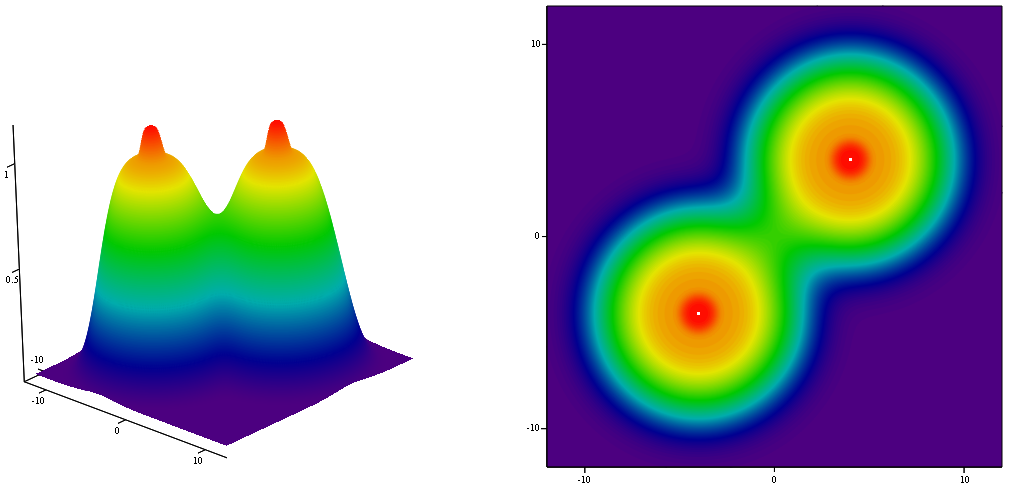
\includegraphics [scale=0.5] {HML_TestFunction_Bosom}
  \caption{Функция Bosom} 
  \label{TestFunctions:img:HML_TestFunction_Bosome}  
\end{figure}

\subsection {Параметры для алгоритмов оптимизации}

\begin{tabularwide}
\textbf{Точность вычислений:} & $\varepsilon=0.06$. \\
\textbf{Число интервалов, на которые предполагается разбивать каждую компоненту вектора $\bar{x}$ в пределах своего изменения} (для алгоритмов дискретной оптимизации) : & $NumberOfParts_j=4095$ ($j=\overline{1,n}$). \\
\textbf{Для этого длина бинарной строки для $x_j$ координаты равна} (для алгоритмов бинарной оптимизации) : & $\left( k_2\right)_j=12$ ($j=\overline{1,n}$). \\
\end{tabularwide}

\textbf{Замечание:}  $NumberOfParts_j$ выбирается как минимальное число, удовлетворяющее соотношению:
\begin{equation*}
NumberOfParts_j=2^{\left( k_2\right)_j }-1\geq\dfrac{10\left( Right_j-Left_j\right) }{\varepsilon},\text{где } \left( k_2\right)_j \in \mathbb{N}, \left( j=\overline{1,n}\right).
\end{equation*}

\subsection {Основная задача и подзадачи}

\begin{tabularwide}
\textbf{Изменяемый параметр: } & $n$ --- размерность вещественного вектора. \\
\textbf{Значение в основной задаче:} & $n=2$.\\
\end{tabularwide}

\subsection {Нахождение ошибки оптимизации}

{\color{red} \textbf{Внимание!} В отличии от других функций формулы нахождения ошибок другие, так как есть несколько идентичных по значению целевой функции глобальных минимумов.}

Пусть в результате работы алгоритма оптимизации за $N$ запусков мы нашли решения $\bar{x}_{submax}^k$ со значениями целевой функции $f\left( \bar{x}_{submax}^k\right) $ соответственно ($k=\overline{1,N}$). Используем три вида ошибок:

\textbf{Надёжность: }
\begin{equation*}
R = \dfrac{\sum_{k=1}^{N}S\left( \bar{x}_{submax}^k \right) }{N}, \text{ где}
\end{equation*}
\begin{equation*}
S\left( \bar{x}_{submax}^k \right)=\left\lbrace \begin{aligned} 1,& \text{ если } \left| \left( \bar{x}_{submax}^k \right)_j-\left( \bar{x}_{max}^1 \right)_j\right|<\varepsilon, j=\overline{1,n};   \\ 1,& \text{ если } \left| \left( \bar{x}_{submax}^k \right)_j-\left( \bar{x}_{max}^2 \right)_j\right|<\varepsilon, j=\overline{1,n};   \\ 0,& \text{ иначе}. \end{aligned}\right.
\end{equation*}

\textbf{Ошибка по входным параметрам:}
\begin{equation*}
E_x = \max_{i=\overline{1,2}} \left\lbrace  \frac{\sum_{k=1}^{N} \left( \frac{\sqrt{\sum_{j=1}^{n}{\left( \left( \bar{x}_{submax}^k \right)_j-\left( \bar{x}_{max}^i \right)_j \right)}^2 }}{n} \right)  }{N}\right\rbrace  .
\end{equation*}

\textbf{Ошибка по значениям целевой функции: } (без изменений)
\begin{equation*}
E_f = \dfrac{\sum_{k=1}^{N} \left| f\left( \bar{x}_{submax}^k \right)-f\left( \bar{x}_{max} \right) \right|  }{N}.
\end{equation*}

\subsection {Свойства задачи}
\begin{tabularwide}
\textbf{Условной или безусловной оптимизации: } & Задача безусловной оптимизации. \\
\textbf{Одномерной или многомерной оптимизации: } & Многомерной (двумерной). \\
\textbf{Функция унимодальная или многоэкстремальная: } & Функция многоэкстремальная. \\
\textbf{Функция стохастическая или нет: } & Функция не стохастическая. \\
\textbf{Особенности: } & Двf одинаковых максимума. \\
\end{tabularwide}

\subsection {Реализация}

Реализация функции взята из библиотеки HarrixMathLibrary в разделе <<Тестовые функции для оптимизации>>, которую можно найти по адресу \href{https://github.com/Harrix/HarrixMathLibrary} {https://github.com/Harrix/HarrixMathLibrary}.

\begin{lstlisting}[caption=Код функции HML\_TestFunction\_Bosom]
double HML_TestFunction_Bosom(double x, double y)
{
/*
Функция двух переменных: функция Bosom.
Тестовая функция вещественной оптимизации.
Входные параметры:
 x - первая вещественная переменная;
 y - вторая вещественная переменная.
Возвращаемое значение:
 Значение тестовой функции в точке (x,y).
*/
double VHML_Result;
double sk1=-((x-4)*(x-4)+(y-4)*(y-4))*((x-4)*(x-4)+(y-4)*(y-4));
double sk2=-((x+4)*(x+4)+(y+4)*(y+4))*((x+4)*(x+4)+(y+4)*(y+4));

VHML_Result=exp(sk1/1000.)+exp(sk2/1000.)+0.15*exp(sk1)+0.15*exp(sk2);
return VHML_Result;
}
\end{lstlisting}

\subsection {Ссылки}

Функция была найдена случайно на развлекательном ресурсе. В качестве тестовой функции замечена не была в литературе.